% vim: set foldmethod=marker foldlevel=0:

\documentclass[a4paper]{article}
\usepackage[UKenglish]{babel}

\usepackage{preamble}

\usepackage{graphicx}
\graphicspath{ {./imgs/} }

\fancyhead[L]{MA139 Assignment 1}
\title{MA139 Analysis 2, Assignment 1}

\begin{document}

\maketitle

\setlength{\parindent}{0em}
\setlength{\parskip}{1em}

% {{{ Q1
\question{1}

Let $\ds S = \sum_{n=1}^\infty \f{x^n}n$. Using the ratio test, we find \begin{align*}
r &= \lim_{n \to \infty} \l| \l. \f{x^{n+1}}{n+1} \r/ \f{x^n}n \r|\\[1ex]
&= \lim_{n \to \infty} \l| \f{x^{n+1} n}{x^n (n+1)} \r|\\[1ex]
&= \lim_{n \to \infty} \l| x \f{n}{(n+1)} \r|\\[1ex]
&= |x| \lim_{n \to \infty} \l| \f{n}{(n+1)} \r|\\[1ex]
&= |x|
\end{align*}
$S$ converges when $r < 1$, so $S$ converges when $|x| < 1$.

Note that the ratio test requires the terms to be nonzero, but the terms of $S$ are only $0$ when $x=0$, and $S$ clearly also converges in this case.

Now we check the edges of the radius of convergence. When $x=1$, $S$ is the harmonic series, which we know diverges. % TODO: Prove this?

When $x=-1$, $S = \sum\limits_{n=1}^\infty (-1)^n \f1n$ and we can use the alternating series test. $\f1n$ is decreasing, non-negative, and converges to $0$, so $S$ must converge by the alternating series test.

Therefore $S$ converges when $-1 \le x < 1$.
% }}}

% {{{ Q2
\newquestion{2}

Let $S = \smlm_{n=1}^\infty a_n x^n$ be the power series in which $a_n = \begin{cases}
1 & \text{if } n \text{ is prime}\\
0 & \text{if } n \text{ is not prime}
\end{cases}$. Then when $0 < x < 1$, $\smlm_{n=1}^\infty a_n x^n < \smlm_{n=1}^\infty x^n = \df1{1-x}$, so $S$ converges. Likewise when $-1 < x < 0$, $\smlm_{n=1}^\infty |a_n x^n| < \smlm_{n=1}^\infty |x|^n = \df1{1-|x|}$, so $S$ converges absolutely. And $S$ trivially converges when $x=0$, so it converges when $-1 < x < 1$. Now we only need to check $x=1$ and $x=-1$.

We know there are infinitely many primes, so $\smlm_{n=1}^\infty a_n \to \infty$. And when $x = 1$, $S = \smlm_{n=1}^\infty a_n$, so $S$ cannot converge.

Note that all prime number except 2 are odd. So when $x = -1$, $S = -1 + 1 + 1 + 1 + \cdots = -1 + \smlm_1^\infty 1$, which clearly diverges to $\infty$.

Therefore, $S$ converges exactly when $-1 < x < 1$.
% }}}

% {{{ Q3
\newquestion{3}

Let $\sum a_n x^n$ be a power series with radius of convergence $R$, let $[-K, K] \subseteq (-R, R)$, and let $f(x) = \smlm_{n=0}^\infty a_n x^n$.

% We will show that $f(x)$ is continuous at all $c \in [-K, K]$. For all $\varepsilon > 0$, we want $\delta > 0$ such that $|x-c| < \delta \implies |f(x) - f(c)| < \varepsilon$.
% \begin{align*}
% |f(x) - f(c)| &= \l| \smlm_{n=0}^\infty a_n (x^n - c^n) \r|\\[1ex]
% &\le \smlm_{n=0}^\infty \l| a_n (x^n - c^n) \r|
% \end{align*}

It was proven in lectures that any convergent power series is continuous in its radius of convergence. Therefore $f(x)$ is continuous in $(-R, R)$ and therefore also in $[-K, K]$.

Since $f(x)$ is continuous in $[-K, K]$, by the extreme value theorem, it is bounded on the interval and attains its bounds.
% }}}

% {{{ Q4
\newquestion{4}

Consider the sequence $\l(\df{\e^n n!}{n^n}\r)$. The ratio of successive terms is \begin{align*}
& \f{\e^{n+1}\, (n+1)!\, n^n}{\e^n\, n!\, (n+1)^{n+1}}\\[1ex]
&= \f{\e\, (n+1)\, n^n}{(n+1)^{n+1}}\\[1ex]
&= \e \l(\f{n}{n+1}\r)^n\\[1ex]
&= \e \l(\f{n+1}n\r)^{-n}\\[1ex]
&= \e \l(\l(1 + \f1n\r)^n\r)^{-1}\\[1ex]
&\to \e \l(\e\r)^{-1}\\[1ex]
&= 1
\end{align*}

The ratio tends to $1$. In particular, $\l(1+\df1n\r)^n$ tends to $\e$ from below, so $\l(1+\df1n\r)^{-n}$ tends to $\df1\e$ from above. Therefore the ratio of successive terms tends to $1$ from above and the ratio is therefore always $\ge 1$, so the terms of the sequence are increasing.

\begin{figure}[h]
	\centering
	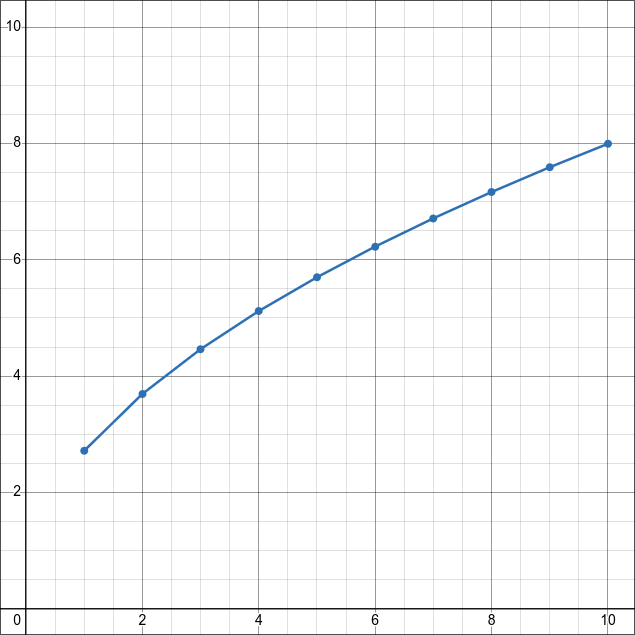
\includegraphics[scale=0.4]{Q4a}
	\caption{The first 10 terms of $\l(\df{\e^n n!}{n^n}\r)$}
\end{figure}

\begin{figure}[h]
	\centering
	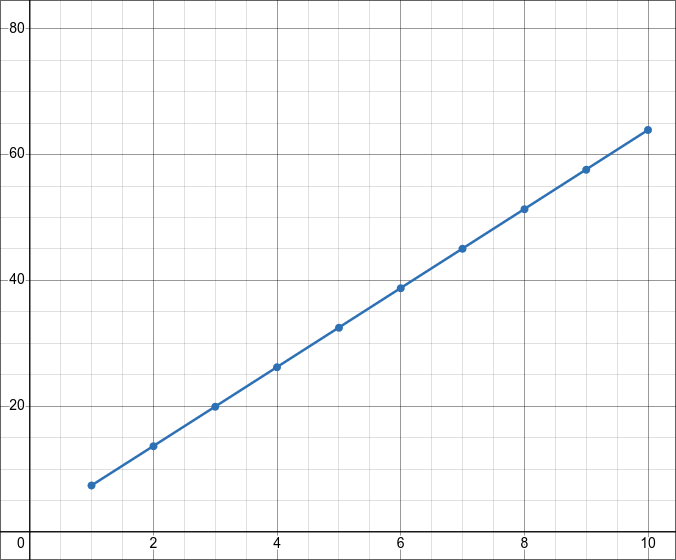
\includegraphics[scale=0.4]{Q4b}
	\caption{The first 10 terms of $\l(\df{\e^n n!}{n^n}\r)^2$}
\end{figure}

The sequence $\l(\df{\e^n n!}{n^n}\r)^2$ looks linear. Experimentally it has a gradient of $6.288747$, which looks suspiciously like $2\pi$. In fact, the line $y = 2\pi x + 1$ fits it almost exactly.

\begin{figure}[h]
	\centering
	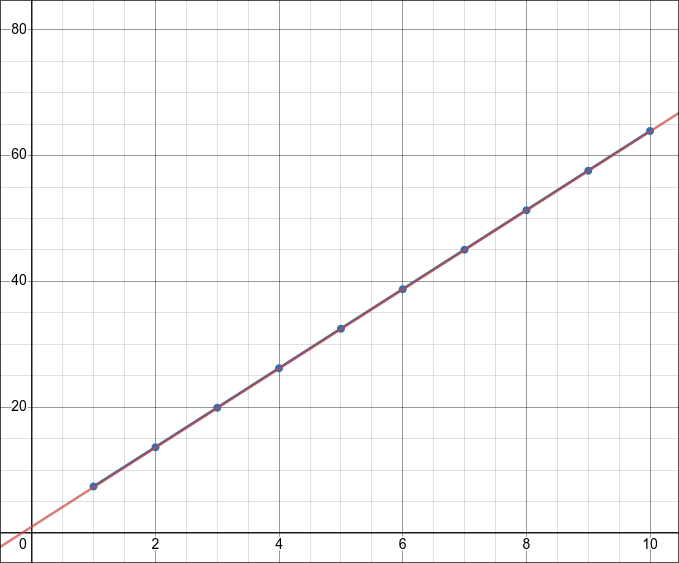
\includegraphics[scale=0.4]{Q4c}
	\caption{$\l(\df{\e^n n!}{n^n}\r)^2$ in blue and $y = 2\pi x + 1$ in red}
\end{figure}
% }}}

\end{document}
